%%
%% This is file `sample-sigconf.tex',
%% generated with the docstrip utility.
%%
%% The original source files were:
%%
%% samples.dtx  (with options: `sigconf')
%% 
%% IMPORTANT NOTICE:
%% 
%% For the copyright see the source file.
%% 
%% Any modified versions of this file must be renamed
%% with new filenames distinct from sample-sigconf.tex.
%% 
%% For distribution of the original source see the terms
%% for copying and modification in the file samples.dtx.
%% 
%% This generated file may be distributed as long as the
%% original source files, as listed above, are part of the
%% same distribution. (The sources need not necessarily be
%% in the same archive or directory.)
%%
%% The first command in your LaTeX source must be the \documentclass command.
\documentclass[sigconf]{acmart}

\usepackage{multicol}

%%
%% \BibTeX command to typeset BibTeX logo in the docs
\AtBeginDocument{%
  \providecommand\BibTeX{{%
    \normalfont B\kern-0.5em{\scshape i\kern-0.25em b}\kern-0.8em\TeX}}}

%% Rights management information.  This information is sent to you
%% when you complete the rights form.  These commands have SAMPLE
%% values in them; it is your responsibility as an author to replace
%% the commands and values with those provided to you when you
%% complete the rights form.
\setcopyright{acmcopyright}
\copyrightyear{2021}
\acmYear{2021}
%\acmDOI{10.1145/1122445.1122456}

%% These commands are for a PROCEEDINGS abstract or paper.
\acmConference[ASD21/22]{The first project delivery of ASD2122}{2021}{Faculdade de Ciências e Tecnologia, NOVA University of Lisbon, Portugal}
\acmBooktitle{The Projects of ASD - first delivery, 2021, Faculdade de Ciências e Tecnologia, NOVA University of Lisbon, Portugal}
%\acmPrice{15.00}
%\acmISBN{978-1-4503-XXXX-X/18/06}


%%
%% Submission ID.
%% Use this when submitting an article to a sponsored event. You'll
%% receive a unique submission ID from the organizers
%% of the event, and this ID should be used as the parameter to this command.
%%\acmSubmissionID{123-A56-BU3}

%%
%% The majority of ACM publications use numbered citations and
%% references.  The command \citestyle{authoryear} switches to the
%% "author year" style.
%%
%% If you are preparing content for an event
%% sponsored by ACM SIGGRAPH, you must use the "author year" style of
%% citations and references.
%% Uncommenting
%% the next command will enable that style.
%%\citestyle{acmauthoryear}

%%
%% end of the preamble, start of the body of the document source.
\begin{document}

%%
%% The "title" command has an optional parameter,
%% allowing the author to define a "short title" to be used in page headers.
\title{High Performance Decentralized Storage System: Implementation and Testing}

%%
%% The "author" command and its associated commands are used to define
%% the authors and their affiliations.
%% Of note is the shared affiliation of the first two authors, and the
%% "authornote" and "authornotemark" commands
%% used to denote shared contribution to the research.
\author{Rodrigo Ribeiro}
\email{rj.ribeiro@campus.fct.unl.pt}
\affiliation{%
  \institution{MIEI DI FCT UNL}
}

\author{João Martins}
\email{jgo.martins@campus.fct.unl.pt}
\affiliation{%
  \institution{MIEI DI FCT UNL}
}

\author{Daniel Batista}
\email{df.batista@campus.fct.unl.pt}
\affiliation{%
  \institution{MIEI DI FCT UNL}
}

%%
%% By default, the full list of authors will be used in the page
%% headers. Often, this list is too long, and will overlap
%% other information printed in the page headers. This command allows
%% the author to define a more concise list
%% of authors' names for this purpose.
\renewcommand{\shortauthors}{Rodrigo Ribeiro, João Martins, and Daniel Batista.}

%%
%% The abstract is a short summary of the work to be presented in the
%% article.
\begin{abstract}
Peer-to-peer systems have been gaining popularity, presenting themselves as a more ``liberal'' alternative to centralization of data backed up by big companies.

One problem of such systems is the location of stored contents. This problem can be solved resorting to distributed hash tables(DHTs). 

In this report we present our implementation of two distinct DHT algorithms with different properties for the purpose of file location. We go over implementation details, parameterization values used, present experimental tests and extract conclusions. Additionally we present some future work related to our project to mention things we could to to improve our solution.
  
\end{abstract}

%%
%% This command processes the author and affiliation and title
%% information and builds the first part of the formatted document.
\maketitle

\section{Introduction}
This project was developed under the \emph{Algorithms and Distributed Systems} course. The goal was to implement two robust and efficient peer-to-peer distributed hash table algorithms and a storage system on top of it to handle file storage functionality for an artificial automated application.

% add motivation
Decentralized storage systems provide a more ``liberal'' alternative to data storage like relying on big companies which have reported leaks and other security risks.  Such systems have been increasing in popularity. One examples of this is FileCoin which raised 250 million dollars with leader investors like Y Combinator, Naval Ravikant, Andreessen Horowitz, Union Square Ventures Sequoia and Winklevoss Capital.

%%%%%%%%%%%%%%%% citar %%%%%%%%%%%%%%%% https://medium.com/bitfwd/what-is-decentralised-storage-ipfs-filecoin-sia-storj-swarm-5509e476995f

\begin{figure}
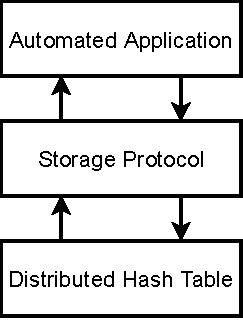
\includegraphics[scale = 0.7]{acmart-master-asd2122/images/ArchitectureOfAProcess.pdf}
\centering
\caption{Architecture of a process.}
\label{fig:processArchitecture}
\end{figure}

The project is composed of three layers which define the architecture of a node. The automated application is responsible for creating artificial store  and retrieve requests of files to the below protocol. The storage protocol is responsible for storing the contents durably and serve them to the Automated Application. Finally, the distributed hash table is responsible for finding the place of a file within the structured overlay of processes.

For this purpose we decided to implement Chord and Kademlia, which happened to be the protocols which had more implementation details and guidance in the literature. We chose to implement these two protocols together since they offer the same functionality, but have different characteristics.

Chord is a very academic example that does not replicate content across multiple nodes in its standard implementation. Kademlia in the other hand supports better node failures, but induces the storage app to store a file in large number of machines.

The development of this project was made in Java and conducted using framework developed in the context of the NOVA LINCS laboratory written by Pedro Fouto, Pedro Ákos Costa, João Leitão, whose internal code-name is Babel.

The structure of this report starts by going over related work, followed by implementation details. After this we present and discuss our experimental results. At the end of the document we present future work to further improve our solution.

\section{Related Work}
In this section we make a brief summary of the theme of the project and provide some context.

At first we present Distributed Hash Tables in abstract and then Chord and Kademlia in specific, which were the ones we implemented. After that we go over decentralized storage systems and after that experimental studies of such systems


\subsection{Distributed Hash Tables}
Distributed Hash Tables aim to provide scalable look up operations for a given key within a peer-to-peer system. 

DHTs use an hash function to assign an id to contents and peers, for example the SHA-1 function which provides 160 bit identifiers. This is called \emph{consistent hashing} and is used to guarantee several properties.

The hash function has a very low probability of collisions, so we assume that if two nodes have the same id, then they are the same node. The same happens with files.

The hash function is also used to assign a content to a peer that will be responsible to store it. We assume that the hash function will assign random values and in that case the probability of a content getting assigned to every host is the same. So in this case the hash function also achieves load balance in the storing of the contents.

One possibility to generate the id of a node is to use the pair ``ipaddress:port'' as the input of the hash function since it will be unique. In order to generate the unique id of a content we can simply perform an hash of the file's name.




% elaborate on dhts

\subsubsection{Chord}
Chord is one of the four original distributed hash-table protocols. It aims to achieve Load Balance, Decentralization, Scalability and Availability, as claimed in the original paper.

Each node gets an identifier using consistent hashing. Using the Chord lookup protocol, nodes and keys are arranged in an circle (a chord) that has at most $2^m$ positions. 

%%%% state of a node
The state of each node is composed of the address of the predecessor node, the successor node and a finger table of addresses of other nodes.

%%%% lookup operation
Upon receiving a lookup operation, a node will find the closest node to the id of the requested content which doesn't surpass it. To find this node it will look to its successor and its finger table and when he finds it will send a FIND-SUCESSOR message to that node.

%%%% stabilize
Periodically Chord requires that a stabilization procedure takes place to keep the pointers up to date with changes in the overlay because nodes can enter and leave the network.


%%%% Where properties are achieved

The core usage of the Chord protocol is to query a key from a client. To ensure correct lookups, the successor pointer of each node must be correct. Therefore, a stabilization protocol is running periodically in the background which updates successor pointers.


As it is described in the original paper Chord isn't really robust in a fault prone environment. We propose improvements to make Chord more robust in section \ref{futureWork}.

\subsubsection{Kademlia}
Kademlia unlike Chord is able to work correctly in a fault prone environment. This is supported by storing each content in up to \emph{k} nodes which will provide redundancy. The mentioned \emph{k}, $\alpha$ and $\beta$ mentioned in the following paragraphs are configuration parameters of the system which can be changed. The values used on our experiments are mentioned in the implementation section \ref{implementation}.

The state kept by each is composed of a set of k-buckets. A k-bucket is a bucket that contains the address and port of up to \emph{k} nodes. These k-buckets are constantly updated with messages exchanged by the protocol, therefore there is no need to create messages to maintain the routing information up to date, like in chord.

In order to perform a lookup, a node will collect the k closest nodes  to the the given id of the request. After that, it will send FIND-NODE messages to $\alpha$ (authors recommend a value of 3) and repeat the process up until its closest k nodes to the lookup id doesn't change.

This last step of checking if all the closest \emph{k} nodes have already been queried happens when a node receives $\beta$ replies (with $\beta < \alpha$). This helps with dealing with delayed replies.


\subsection{Distributed and Decentralized Storage Systems}
Decentralized storage systems consist of a peer-to-peer network of user operators who hold a portion of the overall data, unlike centralized systems that are operated by a single point of failure a decentralized storage systems has more redundancy and is fault-tolerant. 

There are already some working implementations of this protocols that are used by millions of people. The most used and well known protocol is the InterPlanetary File System (IPFS). It was started by Protocol Labs to create a new way to server information on the web. Other example of working implementations are FileCoin, Sia, Storj and Swarm.

\subsection{Decentralized Storage Systems: Use Cases}



\section{Our Solution}\label{implementation}
In the start of the section, provide a quick overview of the section (to assist the reader in understanding the organization)

\subsection{Automated Application}
The Automated application's code was provided and its purpose is to generate requests to store and retrieve random contents to the Storage Protocol.

The application starts by issuing multiple content store requests to the layer below. When the stores have been complete, it starts issuing retrieve operations.

The following parameters can be changed to alter the functioning of the Application layer.

\begin{multicols}{2}
\begin{itemize}
    \item Content number
    \item Payload size
    \item Store time
    \item Retrieve time
    \item Run time
    \item Cooldown time
    \item Request interval
    \item Total processes
\end{itemize}
\end{multicols}

\subsection{Storage Protocol}
This protocol is responsible handling store and retrieve operations from the Automated Application and storing the contents durably.

Upon receiving a store request, the Storage Protocol will query the DHT layer and ask for the node, or best nodes to store a given content. When the layer below replies with the node or best nodes to store the content, in the case of Kademlia, it will store the contents in all of referred nodes, contacting directly their Storage Protocol.

Upon a retrieve request, it will do the same thing again. It will issue a lookup request to the layer below and after that it will search for the contents in the node, or nodes, retrieved by the layer below.

\subsection{Chord}

\subsubsection{Parametrization}

In the chord protocol, three timers can be parameterized: the "chord stabilize interval" and "chord fix finger interval" regulate how frequently the procedures stabilize and fix fingers occur.
The parameter "chord keep alive interval" regulates how frequently messages are sent to keep TCP connections open to membership nodes and also to identify and remove nodes in the membership that are not responding.
The number of participating nodes must be specified in advance in the parameter "number of processes". Our implementation computes the number of fingers by utilizing this parameter in the following equation: 
\[Fingers (n)=2.log_2(n)\]
The size of the node identifier is set at 160 bits. This decision was taken to keep the protocol comparable to Kadmelia. 
The size of the ring cannot be parameterized, it is equal to $2^m$, where m is the size of the id space (160 bits). 
We had to alter the calculation that determines the position of each finger since the size of the ring is no longer dependent on the number of participating nodes. 
\[ fingerPosition_i(np) = ((np + 2^8^0) \% 2^1^6^0) / (Fingers(n) - i) \]
If the standard formula was used, all fingers would point to the same node since the increment in position would be minimal in proportion to the id space.
The 16th finger in a node with the id(2.0e+40) would point to the position $2.0*10^4^0 + 2^1^6$, this position most likely belongs to the successor node. With the suggested formula, the last finger would point 

%chord_keep_alive_interval=4000
%chord_stabilize_interval=1000
%chord_fix_finger_interval=1000
%int numberOfFingers = Math.min(numberOfNodes-1, 2*(int)(Math.log(numberOfNodes) / Math.log(2)));
% finger_position = ((node_position + 2^80) % 2^160) / (number_finger - finger_index)

\subsection{Kademlia}

\subsubsection{Parametrization}
The \emph{k} value specifies the size of each k-bucket and the amount of nodes to reply to the upper layer. We used 5 for this parameter in order to simulate a bigger overlay at scale and to still have a \emph{k} bigger than $\alpha$.

 The $\alpha$ constant defines the number of concurrent queries happening. In our implementation we used a value of 3. This was the value proposed by the authors of the original paper.
 
 The $\beta$ value we used was equal to 1. It specifies the number of FIND-NODE replies we must receive until checking if we contacted all the nodes on our current closest K for that lookup in order to deliver a result to the upper layer.
 

\subsubsection{Messages}
The original paper mentions four Remote Procedure Call (RPC) messages which are the following: PING, FIND-NODE, STORE and FIND-VALUE.

However, in the context of the project and with the process architecture presented in Figure \ref{fig:processArchitecture}, we implemented Kademlia only resorting to PING (and corresponding reply) and FIND-NODE RPCs.

The FIND-VALUE message in the original protocol was replaced by a FIND-NODE in our implementation. This happened because when a node receives a FIND-VALUE message and contains that content locally, it is supposed to return its closest k nodes and the value as well, which wouldn't work on our layered architecture which gives content transfer responsibilities to the storage protocol. So in our implementation we simply wait for the DHT layer to discover the k closest nodes it can and send them to the Storage Protocol which will then contact the k closest nodes to retrieve the files.

The STORE RPC of the original paper is equivalent to a STORE-CONTENT message of the storage protocol in our implementation.



\section{Implementation: What we did}
In this section we mention what happened during the implementation. We justify the features we did and didn't implement.

\subsection{Base Protocol Class}

\subsection{Kademlia}
In this subsection we give relevant details on our Kademlia implementation timeline.

\subsubsection{$\beta$ value}
We used the $\beta$ value of 1 for evaluating our implementation, but we noticed that when testing the algorithm with a value of 2 something blocked and we didn't know what happened. All processes completely froze.

\subsubsection{Population}
We found a master thesis which mentions a bootstrapping population phase that is performed after the FIND-NODE lookup that is sent to the contact node. This step consists of querying all buckets that are to the right (with an higher index) of the first non-empty bucket.

%%%%%%%%%%%%%%%% citar a tese %%%%%%%%%%%%%%%% 

This phase would guarantee that when nodes are added to a overlay with many nodes it knows of nodes that aren't close to him, because we more than the lookup for himself.

We implemented this feature but after delivery noticed it had a bug so we just removed it. This feature also wouldn't have a big impact on the tests we performed because we run few nodes and this nodes know of other nodes that are somewhat far away on the identifier space.


\subsubsection{Ping Messages}
We didn't test the ping message's effects because its very hard to launch enough processes on our local machines to fill one out of 160 buckets completely so we can test it out. Anyway, it should be working fine since it is not a very complex operation to ping a node and proceed or not to alter a bucket.


\section{Experiments}
In our experimental evaluation we deployed 50 nodes across 2 machines on the cluster of the informatics department of the School of Science and Technology. The machines were equal and had 16 cores with 16 threads and 32GB of RAM each.

The following subsections present the results we got for both Chord and Kademlia under four different test settings.



\section{Future Work}\label{futureWork}
During the project's timeline it wasn't possible to implement all our ideas which extended the original descriptions of the DHT algorithms. Anyhow we present some future work that would extend and further improve our solution.

\subsection{Storage Protocol Level Caching of Contents}
This feature would impose the storage protocol to implement a cache of the served files that are not stored locally. This way, when the storage protocol is asked to retrieved a file that he has recently served to the upper layer, it will directly contact the owner of that content instead of querying the DHT layer.

We expect this idea to improve the performance of the system with the right configuration of time-to-leave and cache size. 

\subsection{Chord Replication of Contents}
It can happen that a node goes down in a real world setting
One way to make chord more robust to failures would be to implement redundancy by storing each value multiple times in the DHT so that when a node fails the contents don't get lost.

\subsection{Chord Content Migration of Contents}
We propose also to migrate contents between nodes. This would happen when a node joins a overlay and there are files whose id's that fall under his id and are stored in other node. In this case, even though the contents are stored in the DHT, the lookup operations will fail to answer the correct node.

One way to solve this is to make a node periodically perform a lookup for the id of the contents it is storing. In case the value returned is not himself, then the node will contact the appropriate node and transfer the files, so that they can be found.

\subsection{Kademlia k-buckets periodic updates}
In kademlia, it can happen that a node isn't queried for some time. If this happens it is possible that its routing information (k-buckets) gets outdated. One way of solving this is to periodically perform a lookup for a node within its k-buckets. This way with the message exchange of the protocol the state of the process will get updated to reflect changes in the overlay.

\subsection{Further testing of our Kademlia implementation}
In order to guarantee a better understanding of the behaviour of our implementation we would need to test it with more nodes.

This happens because with the amount of processes we ran, nodes have a its buckets filled with a decent portion of all nodes in the overlay and it is very unlikely to have a bucket with all its \emph{k} entries full with an id space of 160 bytes. So ping messages will be very rare to happen.


\section{Cenas para por na bibliografia}

paper do kademlia
tese do kademlia

paper do chord



%%
%% The acknowledgments section is defined using the "acks" environment
%% (and NOT an unnumbered section). This ensures the proper
%% identification of the section in the article metadata, and the
%% consistent spelling of the heading.
\begin{acks}
To Robert, for the bagels and explaining CMYK and color spaces.
\end{acks}

%%
%% The next two lines define the bibliography style to be used, and
%% the bibliography file.
\bibliographystyle{ACM-Reference-Format}
\bibliography{sample-base}

\end{document}
\endinput
%%
%% End of file `sample-sigconf.tex'.
